% !TEX program = xelatex

%%%%%%%%%%%%%%%%%%%%%%%%%%%%%%%%%%%%%%%%%
% Thin Sectioned Essay
% LaTeX Template
% Version 1.0 (3/8/13)
%
% This template has been downloaded from:
% http://www.LaTeXTemplates.com
%
% Original Author:
% Nicolas Diaz (nsdiaz@uc.cl) with extensive modifications by:
% Vel (vel@latextemplates.com)
%
% License:
% CC BY-NC-SA 3.0 (http://creativecommons.org/licenses/by-nc-sa/3.0/)
%
%%%%%%%%%%%%%%%%%%%%%%%%%%%%%%%%%%%%%%%%%

%----------------------------------------------------------------------------------------
%	PACKAGES AND OTHER DOCUMENT CONFIGURATIONS
%----------------------------------------------------------------------------------------

\documentclass[a4paper, 11pt]{article} % Font size (can be 10pt, 11pt or 12pt) and paper size (remove a4paper for US letter paper)
\usepackage[table]{xcolor}
\usepackage{fontspec}
\definecolor{keycolor}{RGB}{172, 42, 42}
\definecolor{mbleu}{RGB}{64,96,127}
\definecolor{vimvert}{RGB}{46, 139, 87}
\usepackage{hyperref}
\usepackage{placeins} 
% \setmainfont{Avenir Next}
% \setsansfont{Avenir Next}

\usepackage{xeCJK}

\usepackage{geometry}
\geometry{left=2.54cm, top=2.54cm, right=2.54cm, bottom=2.54cm}
\usepackage{subcaption}
\usepackage{tikz}
\usetikzlibrary{tikzmark}
\usepackage{listings}
\usepackage{color}
\usepackage{forest}
\usepackage{float}
\usepackage{makecell}
\usepackage[binary-units]{siunitx}
\usepackage{enumitem}

\lstset{
basicstyle=\small,%
escapeinside=``,%
keywordstyle=\color{blue} \bfseries,% \underbar,%
identifierstyle={},%
commentstyle=\color{blue},%
stringstyle=\ttfamily,%
%labelstyle=\tiny,%
extendedchars=false,%
linewidth=\textwidth,%
numbers=left,%
numberstyle=\tiny \color{blue},%
frame=trbl%
}
 
\newcounter{code}
\lstnewenvironment{code}[3][C++]%
  {%
    \renewcommand\lstlistingname{代码}
    \lstset{% frame=tb,
    language=#1,
    caption=#2,
    label=#3
    }
  }{}

% \usepackage{fancyhdr}
% \usepackage{lastpage}
% \pagestyle{fancy}
% \fancyhf{}
% \fancyfoot[R]{第 \thepage 页,共 \pageref{LastPage} 页}
% % \fancyfoot[C]{\thepage/\pageref{LastPage}}
% \renewcommand{\headrulewidth}{0pt} 
% \renewcommand{\footrulewidth}{0.4pt} 
\renewcommand{\lstlistingname}{Code} % Listing->Code

% \usepackage[protrusion=true,expansion=true]{microtype} % Better typography
\usepackage{graphicx} % Required for including pictures
\usepackage{wrapfig} % Allows in-line images
\usepackage{newfloat}
\usepackage{amsmath}
\usepackage{multirow}

\usepackage{mathpazo} % Use the Palatino font
\usepackage[T1]{fontenc} % Required for accented characters
\linespread{1.2} % Change line spacing here, Palatino benefits from a slight increase by default
% \setlength{\parskip}{0.2em}

\usepackage{indentfirst}
\setlength{\parindent}{2em}

\makeatletter
\renewcommand\@biblabel[1]{\textbf{#1.}} % Change the square brackets for each bibliography item from '[1]' to '1.'
\renewcommand{\@listI}{\itemsep=0pt} % Reduce the space between items in the itemize and enumerate environments and the bibliography

\renewcommand{\maketitle}{ % Customize the title - do not edit title and author name here, see the TITLE block below
\begin{center} % Right align
{\LARGE\@title} % Increase the font size of the title

\large{\@subtitle}

\vspace{1em} % Some vertical space between the title and author name

{\large\@author} % Author name
% \\\@date % Date

% \vspace{1.5em} % Some vertical space between the author block and abstract
\end{center}
}

\renewcommand{\figurename}{图}
\renewcommand{\tablename}{表}

%----------------------------------------------------------------------------------------
%	TITLE
%----------------------------------------------------------------------------------------

\title{\textbf{操作系统实验项目}\\ % Title
} % Subtitle
\newcommand\@subtitle{C与汇编开发独立批处理的内核}

\author{郑戈涵\quad 17338233\quad 931252924@qq.com} % Institution

\date{2020年5月3日} % Date


%----------------------------------------------------------------------------------------

\begin{document}

\maketitle % Print the title section

%----------------------------------------------------------------------------------------
%	ABSTRACT AND KEYWORDS
%----------------------------------------------------------------------------------------

\renewcommand{\abstractname}{摘要} % Uncomment to change the name of the abstract to something else

\begin{abstract}
  本次实验共完成两个任务:使用汇编语言与c语言的混合编程和独立内核的设计与加载
\end{abstract}

% \hspace*{3,6mm}\texttt{Keywords:} lorem , ipsum , dolor , sit amet , lectus % Keywords

\vspace{1em} % Some vertical space between the abstract and first section

\setcounter{tocdepth}{2}
\renewcommand{\contentsname}{目录}
\tableofcontents

% \vspace{2em} % Some vertical space between the abstract and first section

\pagebreak

\section{实验目的}

% 问题、方法、实验目的、意义
\begin{enumerate}
  \item 加深理解操作系统内核概念
  \item 了解操作系统开发方法
  \item 掌握汇编语言与高级语言混合编程的方法
  \item 掌握独立内核的设计与加载方法
  \item 加强磁盘空间管理工作
\end{enumerate}


\section{实验要求}

\begin{enumerate}
  \item 知道独立内核设计的需求
  \item 掌握一种x86汇编语言与一种C高级语言混合编程的规定和要求
  \item 设计一个程序,以汇编程序为主入口模块,调用一个C语言编写的函数处理汇编模块定义的数据,然后再由汇编模块完成屏幕输出数据,将程序生成COM格式程序,在DOS或虚拟环境运行.
  \item 汇编语言与高级语言混合编程的方法,重写和扩展实验二的的监控程序,从引导程序分离独立,生成一个COM格式程序的独立内核.
  \item 再设计新的引导程序,实现独立内核的加载引导,确保内核功能不比实验二的监控程序弱,展示原有功能或加强功能可以工作.
  \item 编写实验报告,描述实验工作的过程和必要的细节,如截屏或录屏,以证实实验工作的真实性
\end{enumerate}

\section{实验内容}

% 输入、输出形式,使用的数据结构,算法的描述,算法正确性说明,算法分析,算法实现所需变量,没有代码
\subsection{分析C程序编译获得的符号列表文档}

\begin{enumerate}
  \item 编译样板C程序,获得符号列表文档.
  \item 分析全局变量、局部变量、变量初始化、函数调用、参数传递情况.
\end{enumerate}

\subsection{汇编和c程序混合编程}

写一个汇编程和c程序混合编程实例,展示你所用的这套组合环境的使用。汇编模块中定义一个字符串,调用C语言的函数,统计其中某个字符出现的次数(函数返回),汇编模块显示统计结果。执行程序可以在DOS中运行.

\subsection{扩展内核程序}

\begin{enumerate}
  \item 把监控程序从引导程序分离独立,生成一个COM格式程序的独立内核,在1.44MB软盘映像中,保存到特定的几个扇区.
  \item 扩展监控程序命令处理能力.
  \item 重写引导程序,加载COM格式程序的独立内核.
\end{enumerate}

\section{实验原理}
\subsection{实模式和保护模式}

\paragraph{实模式}  \cite{wikirmode}
实模式(英语:Real mode)是Intel 80286和之后的x86兼容CPU的操作模式。实模式的特性是一个20比特的区段存储器地址空间(意思为只有1 MB的存储器可以被定址),可以直接软件访问BIOS例程以及周边硬件,没有任何硬件等级的存储器保护观念或多任务。

\paragraph{实模式的缺陷}\cite{realmodedownside}
\begin{itemize} 
  \item 实模式下操作系统和用户程序属于同一特权级,这哥俩平起平坐,没有区别对待。
  \item 用户程序所引用的地址都是指向真实的物理地址,也就是说逻辑地址等于物理地址,实实在在地指哪打哪。
  \item 用户程序可以自由修改段基址,可以不亦乐乎地访问所有内存,没人拦得住。
  以上3个原因属于安全缺陷,没有安全可言的CPU注定是不可依赖的,这从基因上决定了用户程序乃至操作系统的数据都可以被随意地删改,一旦出事往往都是灾难性的,而且不容易排查。
  \item 访问超过64KB的内存区域时要切换段基址,转来转去容易晕乎。
  \item 一次只能运行一个程序,无法充分利用计算机资源。
  \item 共20条地址线,最大可用内存为1MB,这即使在20年前也不够用。
\end{itemize}

\paragraph{保护模式}\cite{wikipmode}
是一种80286系列和之后的x86兼容CPU的运行模式。保护模式有一些新的特性,如存储器保护,标签页系统以及硬件支持的虚拟内存,能够增强多任务处理和系统稳定度。现今大部分的x86操作系统都在保护模式下运行,包含Linux、FreeBSD、以及微软Windows 2.0和之后版本。

\paragraph{虚拟8086模式}  \cite{wikiv8086}
在80386微处理器及更高版本中,虚拟8086模式(也称为虚拟实模式,V86模式或VM86)允许执行实模式应用,这些实模式应用无法在处理器运行保护模式操作系统时直接在保护模式下运行。 它是一种硬件虚拟化技术,它允许386芯片模拟多个8086处理器。 它源于80286保护模式的痛苦经历,它本身并不适合很好地运行并发实模式应用程序。

\subsection{函数调用约定}

函数调用约定是什么?
调用约定,calling conventions,从字面上理解,它是调用函数时的一套约定,是被调用代码的接口,
它体现在:
\begin{itemize} 
  \item 参数的传递方式
  \item 参数的传递顺序
  \item 寄存器环境是调用者保存,还是被调用者保存,保存哪些寄存器
\end{itemize}
\paragraph{X86调用约定}
cdecl(C declaration,即C声明)是源起C语言的一种调用约定,也是C语言的事实上的标准(本次实验采用该约定)。在x86架构上,其内容包括:
\begin{itemize} 
  \item 函数实参在线程栈上按照从右至左的顺序依次压栈。
  \item 函数结果保存在寄存器EAX/AX/AL中
  \item 浮点型结果存放在寄存器ST0中
  \item 编译后的函数名前缀以一个下划线字符
  \item 调用者负责从线程栈中弹出实参(即清栈)
  \item 8比特或者16比特长的整形实参提升为32比特长。
  \item 受到函数调用影响的寄存器(volatile registers):EAX, ECX, EDX, ST0 - ST7, ES, GS
  \item 不受函数调用影响的寄存器: EBX, EBP, ESP, EDI, ESI, CS, DS
  \item RET指令从函数被调用者返回到调用者(实质上是读取寄存器EBP所指的线程栈之处保存的函数返回地址并加载到IP寄存器)
\end{itemize}

\subsection{保护模式的运行模式反转}
CPU 处于实模式下时,并不是变成了纯粹的 16 位 CPU,它相当于 8086 的加强版,依然可以使用 32 位下的资源。也就是说,资源是共通的,无论哪种模式都可以在指令中使用它们,同样一句汇编代码,
编译器无法确定它到底是属于实模式,还是属于保护模式呢,需要人为告诉编译器一些信息:

\begin{itemize} 
  \item [bits 16]是告诉编译器,下面的代码帮我编译成 16 位的机器码。
  \item [bits 32]是告诉编译器,下面的代码帮我编译成 32 位的机器码。
\end{itemize}

\subsection{混合注意事项}
\begin{itemize} 
  \item 编写混合的代码时,跳转部分要尤其注意,包括跳转和返回,\textit{nasm}支持\textit{call dword}和\textit{retf}语句,调用c函数时使用\textit{call dword}能够在跨段时保存CS和IP到栈中,调用汇编的过程时使用\textit{retf}能够在返回时弹出CS和IP,正确跨段返回。
  \item 由于函数语句执行时会破坏原有环境,在每次进入汇编时都需要使用\textit{pusha}将所有常用寄存器入栈,离开汇编时使用\textit{popa}将所有常用寄存器出栈。
  \item 不能在传入char*类型变量时使用字面量字符串,比如print("Message")这样的,使用后可能出现下图的错误:read\_virtual\_checks():read   beyond limit.
\end{itemize}

\begin{figure}[H]
  \centering
  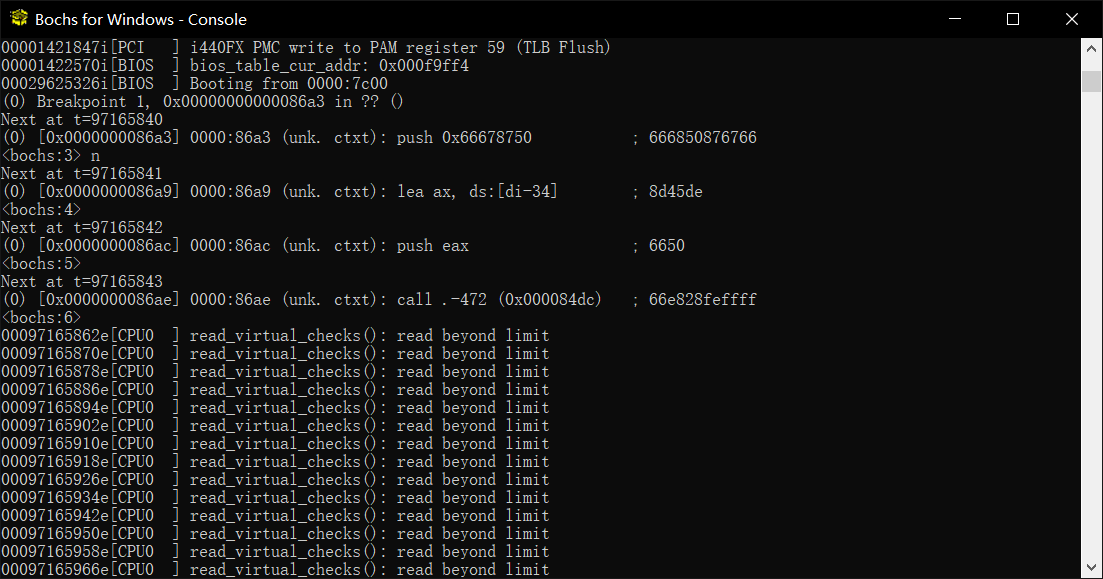
\includegraphics[width=0.8\linewidth]{strerror.png}
  \caption{传入字面值字符串参数}
  \label{fig:mixtest}
\end{figure}


\section{实验过程}

本次实验考虑到\textit{dosbox}和\textit{tcc,tasm,tlink}上手比较复杂,因此使用了\textit{gcc,nasm,ld}。
由于出现了内核程序,这次实验开始将会在实模式和保护模式上有较大差别,我将使用实模式完成实验。
\begin{enumerate}
  \item 编写汇编程序和c程序,生成镜像并测试
  \item 修改引导程序,只加载内核程序,并跳转
  \item 设计c库和汇编库,封装基本的io操作
  \item 修改监控程序,扩展功能
  \item 设计用户程序的加载方式
  \item 修改用户程序
  \item 生成镜像,在虚拟机中加载
\end{enumerate}
\subsection{混合编程}

我设计的样板c程序将同时用于符号列表文档分析和测试混合编程
\subsubsection{分析c程序汇编结果}

生成汇编文件可以使用下面的两种方法,第一种方是通过\textit{objdump}生成,比较清晰,简单,第二种包含了\textit{gcc}产生的附加信息,比较复杂。
\begin{code}{生成汇编文件}{code:generateasm}
# 方法一
gcc -fno-pie -c -m16 -march=i386 -nostdlib -ffreestanding 
-mpreferred-stack-boundary=2 -lgcc -shared str.c -o str.o
objdump  -s -ld -C -S str.o > str.s
# 方法二
gcc -fno-pie -c -m16 -march=i386 -nostdlib -ffreestanding 
-mpreferred-stack-boundary=2 -lgcc -shared str.c -S -o str.o
\end{code}
下面对\textit{gcc}编译产生的文件进行分析,首先是比较简短的c语言代码:
\begin{lstlisting}[language={c},label=str_c,caption=str.c]
  extern void cls();
  extern void putchar(char c);
  extern void printPos(char *str, int n, int row, int col);
  char *msg = "wodemsg1";
  int strlen(char *str)
  {
    int cnt = 0;
    while (str[cnt++] != '\0')
      ;
    return cnt-1;
  }
  void printInfo()
  {
    cls();
    char *Info = "wodeinfo";
    putchar(strlen(Info)+ '0');
    printPos(Info, strlen(Info), 6, 23);
    printPos(msg, strlen(msg), 9, 23);
  }
  
  void printmsg(){
    int row = 9, col=23;
    printPos(msg, strlen(msg), row, col);
  }
  \end{lstlisting}
程序完成了简单的两个功能,计算字符串的长度和打印两个字符串到屏幕上。
为节省篇幅,我去掉了两个比较复杂的函数,代码请看\ref{str.o},\textit{gcc}生成的汇编文件中分了非常多的部分,在开头有标签(如\textit{.LC0 :}),后面引用时会用此名字引用。
\paragraph{全局变量}
全局的变量前面都有\textit{.globl}标签,比如第4行的msg,在链接之后生成的文件里,汇编的代码也是能够调用这些变量的。

\paragraph{函数调用}
函数声明也是有标签的,比如29行的printmsg。在32行,函数将ebp压栈,35行将esp传给ebp,使用ebp作为基址进行寻址。37行将esp向下移动8个字节,
完成局部变量的空间分配。然后38,39两句movl将栈中分配的局部变量进行初始化,分别赋值9和23。40行将msg的地址取到eax中并压栈,
这样子就完成了strlen调用时的参数传递。42行调用strlen过程。接下来的分析基本相同。

\subsubsection{混合编程程序设计}
混合编程中,c代码若要使用汇编的函数,需要使用extern声明此函数,汇编代码中需要在开头将其声明为global;汇编代码若要使用c的函数,需要用extern 关键字
为了体现混合编程的优势,代码里面使用了汇编调用c函数的方法和c函数调用汇编的方法。最后\textit{test.asm}里面直接调用这些过程。
\textit{printpos}函数定义在str.c\ref{str_c}中。注意c语言的函数调用约定,通过栈基址寄存器bp获得参数。

\textit{test.asm}中只调用了\ref{str_c}中的\textit{printmsg}函数。

接下来使用Makefile生成test.img。
\begin{code}{生成测试镜像文件}{code:generateimg}
make testimg
\end{code}

用bochs运行,bochs的配置可以参考附录。使用bochs的原因是vmware在这次实验中的显示出现不少问题,bochs均能正常显示。

\begin{figure}[H]
  \centering
  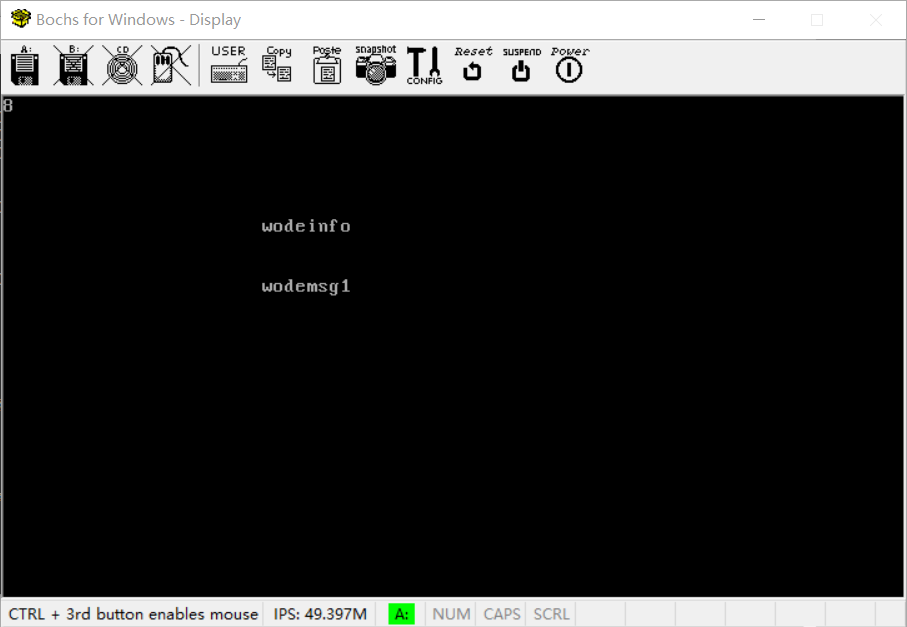
\includegraphics[width=0.8\linewidth]{mixtest.png}
  \caption{运行过程截图}
  \label{fig:mixtest}
\end{figure}

\subsection{修改引导程序}
在上一次实验中,我已将内核从加载程序中独立出来,但是引导程序中将四个用户程序预先加载到了内存中,按照我的设计,用户程序由用户自己载入并运行,因此引导程序中去掉那四个加载扇区的代码即可,这里不放出代码。
由于内核需要丰富的功能,而汇编相对于c语言难以实现复杂功能,因此虽然我使用了汇编文件作为内核,引导程序将跳转至此,但是内核文件仅完成两件事
\begin{enumerate}
  \item 打印欢迎语句
  \item 在用户按下回车键后跳转到c程序中
\end{enumerate}
获得输入用到了BIOS的16号0功能调用,代码来自上次实验。整个内核的代码如下:
\begin{lstlisting}[language={[x86masm]Assembler},label=kernel.asm,caption=kernel.asm]
BITS 16
extern Greet
extern shell

global _start
_start:
    call dword Greet
WaitForKey:
    mov ah, 0
    int 16h
    cmp al, 0dh   
    jne WaitForKey
    call dword shell
    jmp WaitForKey
\end{lstlisting}
  

\subsection{设计库过程}

由于此次项目的函数较多,为了更加清晰的说明函数的设计,附录中给出了库中用到的变量表\ref{tab:varlist}。
所有c代码均放在mystring.h,汇编代码均放在lib.asm中,交互模块所用的函数在interface.h中。

为了让内核有更加丰富的功能,首先要让io操作能够容易进行,也就是封装。
io操作包括输入和输出,这两项依赖于汇编,在建立了基本io操作的基础上,需要c语言来完成简单的字符串操作。

\subsubsection{获得输入}
获得输入是bios调用的基本操作,直接使用调用16号中断即可,代码请看\ref{getch}

\subsubsection{拆分字符串}
该函数用于解析用户的输入,通过遍历字符与空格比对,将对应字符分别赋值到传入的字符串地址中。代码请看\ref{split}

\subsubsection{比较字符串}
该函数用于解析用户的输入,用通过遍历字符直到找到'$\backslash$0'或不同的字符,将此处的字符ASCII码之差返回。代码请看\ref{strcmp}

\subsubsection{计算字符串长度}
该函数在测试部分已实现,请参考\ref{str_c}

\subsubsection{输出字符串}
输出字符串有两种,分别是在特定位置输出,用于打印欢迎页面等一次性功能,另一种是在光标处输出,这种用的最多。
第一种和老师之前提供的代码没有太大差异,注意按照\_cdecl的调用约定,所有变量在压栈时使用4个字节,pusha压栈8个寄存器,共16个字节。
代码同\ref{putchar}。

\subsubsection{输出字符}
输出字符只需考虑光标处,使用BIOS的10号0E功能中断。代码如下:
\begin{lstlisting}[language={[x86masm]Assembler},label=putchar,caption=putchar]
putchar:
    pusha
    mov bp,sp
    add bp,16+4
    mov al,[bp]
    mov bh,0
    mov ah,0Eh;功能码
    int10h
    popa
    retf
\end{lstlisting}

\subsubsection{清屏}

清屏是交互界面必须的功能,调用BIOS的10号3中断完成。
代码如下:
\begin{lstlisting}[language={[x86masm]Assembler},caption=字符串输出宏]
  cls:
  pusha
  mov ax, 0003h
  int 10h
  popa
  ret
  
\end{lstlisting}
以上便是此次实验需要的所有字符相关的IO功能。

\subsection{监控程序修改}

现有的监控程序只能输入四个字符,为了扩展,我模仿了zsh的界面,能够获取用户输入的命令。进入界面时会输出欢迎用的字符串,
等待输入时会打印“->”字符。我添加了三个函数,分别是读取输入的readbuff和greet和prompt。后两个只是调用写好的printpos直接输出字符串,所以不作说明。

\subsubsection{获得输入--readbuff函数}
由于BIOS并没有提供获取键盘输入同时显示对应字符并控制光标的功能,需要自己实现,读取时总共有三种情况,

\begin{enumerate}
  \item 缓冲区中有字符(串)
  \item 缓冲区已满
  \item 缓冲区为空
\end{enumerate}
首先检查传入的字符串是否为空,初始化缓冲区长度变量,然后用定义好的getch获得字符。接下来进入循环。

\paragraph{循环体内}
首先检查是否输入了非法字符,按照三种情况依次判断。合法字符为键盘上可以显示为字符的键和回车,空格,退格和ctrl-c。
若为非法字符重新开始循环,离开循环。若为回车,将字符串长度置为零,代表之前的输入无效,然后离开循环。

\subparagraph{缓冲区中有字符(串)}
若输入的字符是退格,则按顺序输出退格空格退格,理由是退格会使光标退后而空格才会改变屏幕上的内容。
不为退格则显示输入的字符,并将字符放入缓冲区,修改缓冲区长度加一。
\subparagraph{缓冲区已满}
此时只能退格,处理方式请参考第一段。
\subparagraph{缓冲区为空}
此时只能输入,处理方式请参考第一段。

\paragraph{离开循环体}
此时需要换行,分别输出'$\backslash$r','$\backslash$n',已达到换行的效果。'$\backslash$n'并不会将光标放回屏幕左侧。代码如下:

\begin{lstlisting}[language={c},label=readbuff,caption=readbuff]
void readbuff(char *buff, int maxLength)
{
    if (!buff)
      return;
    int len = 0;
    while(1) {
        char c = getch();
        if(!(c==0xD || c=='\b' ||c==3|| c>=32 && c<=127)) { continue; }  
        if(c==0x0D){
            break;
        }
        else if(c==3){
            len = 0;
            break;
        }
        if(len > 0 && len < maxLength-1) { 
            if(c == '\b') {  
                putchar('\b');
                putchar(' ');
                putchar('\b');
                --len;
            }
            else{
                putchar(c);  
                buff[len] = c;
                ++len;
            }
        }
        else if(len >= maxLength-1) {  
            if(c == '\b') {  
                putchar('\b');
                putchar(' ');
                putchar('\b');
                --len;
            }
        }
        else{  
            if(c != '\b') {
                putchar(c);  
                buff[len] = c;
                ++len;
            }
        }
    }
    putchar('\r'); putchar('\n');
    buff[len] = '\0';  
}
\end{lstlisting}
  

\subsubsection{其他功能}
为了完善交互体验,本程序提供关机功能,本质上是通过写端口实现的,代码如下:

\begin{lstlisting}[language={[x86masm]Assembler},caption=强制关机]
shutdown:
    mov ax, 2001H
    mov dx, 1004H
    out dx, ax
  \end{lstlisting}
  

\subsubsection{交互模块--shell函数}

shell函数负责循环获取用户输入并处理。该监控程序提供了五个功能,分别是:
\begin{enumerate}
  \item help:提示用户可以输入的内容
  \item cls:清屏
  \item shutdown:关机
  \item run:运行程序
  \item ls:显示可运行的程序信息
\end{enumerate}
这几个功能被定义为枚举类型,并且有对应的字符串数组用于存放名字以与用户输入比对。函数开头还定义了用户输入缓冲区,命令字符串和目标字符串。
以及用于处理ctrl-c的空字符串,专门使用局部变量存放的理由是,整个项目中无法使用常量字符串,理由未知。使用后会访问不可访问的地址导致死机。

\subsubsection{交互逻辑}
进入循环前清屏,在循环开始时打印提示符“->”,然后使用\textit{readbuff}函数获得输入,依次与commands中的字符串使用\textit{strcmp}比对,
相等时调用对应的功能函数。而最后要判断是否输入了run,是则检查输入的格式,格式用正则表达式可以表示为“run$\backslash$s+[1234]+”,如果格式符合,则进行处理。
处理过程请看下一节。


\subsection{设计用户程序的加载方式}
由于时间原因,我设计的加载方式是用户能够通过命令按照自己输入的数字顺序自动运行程序。

为了使用户能够看到可以加载的程序信息,我定义了结构体\textit{sector},和对应的数组\textit{Comlist}用于装程序的信息。
在检查run命令的格式正确后,\textit{target}字符串中放入了代表运行顺序的数字串,用for循环依次将其转为数字并调用运行函数。
\subsubsection{运行用户程序--loadUsrProgram}
该函数定义在汇编代码中,传入的参数分别是程序的柱面号,磁头号,起始扇区号,扇区数,起始扇区号等信息,调用时这些信息都在栈里,
加载用户程序的代码参考老师第二次提供的引导代码,调用的参数偏移量依次加4,读入扇区后,需要跳转到程序中运行。
这里有三个编程时非常需要注意的点:
\paragraph{堆栈的对齐}
由于使用的是c语言的\_cdecl的调用约定,参数的栈空间释放工作由c语言编译出来的汇编完成,但是call和ret这样隐式压栈和出栈需要汇编自己安排,
考虑到可能会出现跨段的问题,我使用了call far,call dword,ret,那么每次都以四个单位入栈和出栈CS和IP是没有问题的,由于程序有一定的代码量,
编写代码者必须保证每个过程对栈的空间维护都是统一的。
\paragraph{远调用}
在进入该函数前,用户程序目前并未放入内存,而所有信息都作为参数被传入,所以进入用户程序时需要自己手动计算段地址和偏移地址,并使用call far指令跳转,
这是唯一能够直接同时修改CS,IP并且地址能够来自内存的指令。地址可以来自内存意味着是可变的,只要在下方定义一个四字节的变量,在函数进行时用参数为其赋值,
就能用来作为call far的参数,这里还有一点需要注意,call far会从参数中分离出CS(后两个字节),IP(前两个字节),而传入的参数是一个完整的四字节偏移地址(例:0x0A100),
需要用寄存器将其分离并移位得到段寄存器,计算公式为
\begin{equation}
  ds=([bp+20]>>4)-10
\end{equation}
其中[bp+20]是传入的第一个参数,因为pusha压栈了16个字节。
得到后将两个参数分别放入内存中名为\textit{program}的地址处,注意前两个字节是IP,后两个字节是CS。然后call far [program],
这样就通过间接寻址完成远调用。

\paragraph{段寄存器的保护}
由于运行用户程序的时候有跨段,而用户程序中是否修改了段寄存器是无法知道的,因此在从用户程序返回时,需要将ds,es复原,否则之后的程序将无法从数据段取出正确数据。
复原的方式可以有两种,压栈然后出栈,或者直接在用户程序返回后将cs借ax赋值给ds和es,我使用的是第二种方法。

注意好以上三点,便可以写出正确的代码。代码请看\ref{loadUsrProgram}:

\subsection{修改用户程序}
用户程序和第二次的基本一致,唯一的区别在于程序开始时将常用寄存器压栈,离开时出栈,返回时使用retf。

\subsection{软盘扇区安排}

因为现在的用户程序由内核来加载,只需要将程序放入镜像的正确位置就可以了。安排请看表\ref{tab:sectortable}:
\FloatBarrier
% Please add the following required packages to your document preamble:
% \usepackage[table,xcdraw]{xcolor}
% If you use beamer only pass "xcolor=table" option, i.e. \documentclass[xcolor=table]{beamer}
\begin{table}[]
  \caption{软盘扇区安排}
  \label{tab:sectortable}
  \begin{tabular}{llll}
  \rowcolor[HTML]{FFFFFF} 
  {\color[HTML]{333333} \textbf{磁头号}} & {\color[HTML]{333333} \textbf{扇区号}} & {\color[HTML]{333333} \textbf{扇区数(大小)}} & {\color[HTML]{333333} \textbf{内容}} \\
  \rowcolor[HTML]{FFFFFF} 
  {\color[HTML]{333333} 0}            & {\color[HTML]{333333} 1}            & {\color[HTML]{333333} 1(512 B)}         & {\color[HTML]{333333} 引导程序}        \\
  \rowcolor[HTML]{FFFFFF} 
  {\color[HTML]{333333} 0}            & {\color[HTML]{333333} 2$\sim$17}    & {\color[HTML]{333333} 16(8 KB)}         & {\color[HTML]{333333} 操作系统内核}      \\
  \rowcolor[HTML]{F8F8F8} 
  {\color[HTML]{333333} 1}            & {\color[HTML]{333333} 1$\sim$2}     & {\color[HTML]{333333} 2(1 KB)}          & {\color[HTML]{333333} 用户程序1(LU.com)}       \\
  \rowcolor[HTML]{FFFFFF} 
  {\color[HTML]{333333} 1}            & {\color[HTML]{333333} 3$\sim$4}     & {\color[HTML]{333333} 2(1 KB)}          & {\color[HTML]{333333} 用户程序2(LD.com)}       \\
  \rowcolor[HTML]{F8F8F8} 
  {\color[HTML]{333333} 1}            & {\color[HTML]{333333} 5$\sim$6}     & {\color[HTML]{333333} 2(1 KB)}          & {\color[HTML]{333333} 用户程序3(RU.com)}       \\
  \rowcolor[HTML]{FFFFFF} 
  {\color[HTML]{333333} 1}            & {\color[HTML]{333333} 7$\sim$8}     & {\color[HTML]{333333} 2(1 KB)}          & {\color[HTML]{333333} 用户程序4(RD.com)}      
  \end{tabular}
  \end{table}
\subsection{镜像文件生成}


使用gcc生成c源文件对应的汇编,nasm生成内核汇编源文件和库过程汇编源文件的elf格式的汇编,使用ld链接可以生成二进制文件,
将引导程序,内核程序和用户程序放入镜像中的合适位置即可生成镜像。

代码相关信息请看readme.md。

在wsl或linux的shell中执行\textit{make all/make img}即可生成镜像(.img)文件,在VMware中加载该镜像,查看结果。到此,实验结束。

\section{程序使用说明}
\subsection{实验环境}

\subsubsection{VMware Workstation 15}
VMware Workstation是VMware公司推出的一款桌面虚拟计算软件,具有Windows、Linux 版本。此软件可以提供虚拟机功能,使计算机可以同时运行多个不同操作系统。此次实验中用于运行镜像文件。
\subsubsection{nasm 2.13.02}
Netwide Assembler 是一款基于英特尔 x86 架构的汇编与反汇编工具。在此次实验中用生成二进制文件(.bin)
\subsubsection{wsl}
本次实验中用到了shell文件以批处理源代码生成镜像,整合于windows系统的wsl能够很方便的处理在windows系统上生成的文件。
\subsubsection{VSCode 1.44.2}
vscode能够方便的使用wsl和latex的pdf生成功能。加载虚拟机以外的所有任务都可以通过vscode完成。
% 如何编译和使用程序

\subsection{编译方法}

\subsubsection{系统要求}

生成镜像文件时,可以使用linux操作系统或者带wsl的windows系统。

\subsubsection{编译过程与参数}

在源代码目录下使用wsl,执行下列代码即可得到镜像文件os17338233.img。
\begin{code}{生成镜像}{code:generateos}
make img
\end{code}

\subsection{运行与演示}
由于篇幅原因,演示部分将主要放在已录制好的OSdemo.mkv中。
进入内核的界面如图 \ref{fig:run} 所示。

\begin{figure}[H]
  \centering
  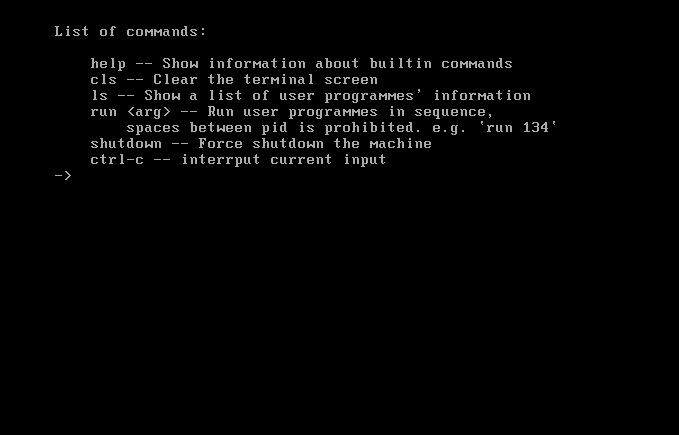
\includegraphics[width=0.8\linewidth]{shell1.png}
  \caption{运行过程截图}
  \label{fig:run}
\end{figure}
具体的演示过程可以查看已录制好的OSdemo.mkv
\section{总结与讨论}

% 特色、问题、教训、改进、收获


\subsection{特色,不足与改进}

本程序提供了较为简洁可用的命令行,支持用户自己载入并按照自己指定的顺序运行程序。为了避免用户恶意修改用户程序的地址,我没有提供修改用户程序信息的功能,
命令行能够为用户提供相对清晰的信息。不足之处是用户程序信息是自己手动写入,无法自动扫描。
\subsection{收获}

本次实验是非常考验汇编和c的编程能力的,尤其是在debug方面,由于汇编会修改上下文,而c用到了很多底层IO操作,汇编后又不容易看出代码结构,
因此单元测试各个模块尤其重要。这次实验我不仅掌握了混合编程的约定,也加强了c的字符串操作的编程能力,还加深对c语言编译后的汇编文件的理解。
此次实验我也学习了如何编写Makefile文件\cite{makefile},大大提高了生成项目目标的效率。最大的收获是关于bochs,在同学的帮助下,
我学会了如何使用bochs对内核进行调试,重要的问题都通过bochs解决。解决的例子会在感想中说明。
同时,在本报告的编写过程中,我也练习了利用 \LaTeX 编写文档的能力。\cite{lamport94, cite}

\subsection{感想}
\paragraph{}
作为操作系统的第三个实验,代码量和第二次相比又有较大的增加,并且完成的功能也更加复杂,要自学的东西翻了好几倍,包括环境配置,编译和链接的方法,
混合编程的约定,以及内核的调试。
\paragraph{}
由于网上的资料并没有特别详细的介绍如何生成裸机使用的二进制文件,编译链接的方法我是通过不断尝试并与同学交流才知道的。
\paragraph{}
实验的每个步骤我都遇到了不少问题,除了与同学探讨外,《操作系统真象还原》\cite{realmodedownside}这本书也提供了非常大的帮助,对我对汇编,调用约定以及实模式,保护模式的理解都有非常大的帮助。
里面关于bochs的演示过程激励我学习bochs的使用方法,在同学的帮助下,我也掌握了bochs的调试方法。可以说,这次实验除非把所有汇编和c的原理都完全吃透,
否则内核调试几乎是必须的,因为代码量太大。仅仅看到虚拟机的显示结果是几乎不能看出问题的。
\paragraph{}
在写混合编程测试代码时,我就遇到了一个严重的问题,所有代码都没有问题,但是vmware虚拟机显示不正确,与同学探讨后才得知,vmware运行某些镜像会有问题,而bochs不会,
我尝试改用bochs运行,果然就没有遇到。但是后面我完成整个项目后,在vmware上也是能正常显示的,目前并不知道原因。
\paragraph{}
通过混合编程理解了调用约定后,完成整个项目的大体工作只花了数小时。其中时间主要花在读取用户输入上,由于我之前对各种逃逸字符的理解还不到位,
运行镜像发现屏幕并没有按照我的想法来显示,查找了相关资料才改正过来。
\paragraph{}
最大的问题毫无疑问是用户程序的加载,这部分是纯汇编代码,由c语言传入结构体的各个分量后调用,我花了大约一整天的时间来解决这个问题,由于代码的问题分散在三处,
在我使用bochs之前,我尝试修改了也没法获得正确的结果,所以我在凌晨时才决定使用bochs进行调试,之所以之前没有使用,是因为bochs中出现了过多c编译产生的汇编代码,阅读起来及其费力,
与objdump生成的文件不同,bochs的反汇编完全不显示所在的模块,因此一旦离开我熟悉的纯汇编代码,cpu执行的语句是属于哪个模块我都无法确定。因此在我决定使用bochs。
bochs的调试方式和gdb相似,在windows系统上有单独的版本。为了运行镜像,首先需要设置配置文件,包括镜像路径,磁盘类型等,然后运行bochsdgb。配置文件可以在src目录下找到。
\paragraph{调试过程}
我首先在0x8100(内核程序起点)处设置断点,并使程序执行到此,然后反汇编了约1400行代码(图\ref{fig:bochsdbg1}),搜索到纯汇编所在的位置(图\ref{fig:bochsdbg2})(图\ref{fig:bochsdbg3}),
在汇编代码开头设置断点(图\ref{fig:bochsdbg4}),继续,然后在窗口中输入命令执行。然后查看所有寄存器的值,包括段寄存器(图\ref{fig:bochsdbg5})。然后设置断点到retf语句,再次检查,
发现段寄存器在retf前已经被修改了,再次设置汇编程序开头为断点,继续,执行到第二个程序时,查看段寄存器,依旧是被修改过的状态,这样就知道了其中有一个问题在于cs,
而两次检查时发现了一个新问题,那就是栈顶sp发生了变化,差距为2,于是我重新启动bochs,在执行完第一个程序后,停留在返回的ret语句,并开始逐步运行代码后,然后将代码复制出来,
与gcc生成的文件通过objdump反汇编得到的文件一一比对语句,终于找到了对应的模块。之所以这么做,是因为我当时并不能确定离开了汇编后是否执行了下一条语句,
可能是因为vmware的问题,我在调用loadUsrProgram后面即使加上了输出字符串的语句,在虚拟机中也没有显示。比对后得知进入了cls模块。于是我发现在调用纯汇编代码cls的子过程返回时,
栈顶并未正常恢复,是因为代码没有使用retf。修改后终于正常运行了程序。而第三个问题是我的ls,我发现执行了汇编的代码后,我的全局变量居然被修改了,而我的汇编代码中并没有访问到全局变量,
使用的都是压栈的参数,c中也只是传入参数后调用了函数而已。于是我将全局变量修改为const,终于解决了所有问题。
\paragraph{}
实际的实验过程远比上述过程所说的复杂,因为如何找到c语言中的对应模块和寻找我所写的纯汇编代码的方法并不是一开始就知道,而是不断摸索才发现可以这么做的。
相信这次实验的收获会对以后的实验有很大的帮助。

\begin{figure}[H]
  \centering
  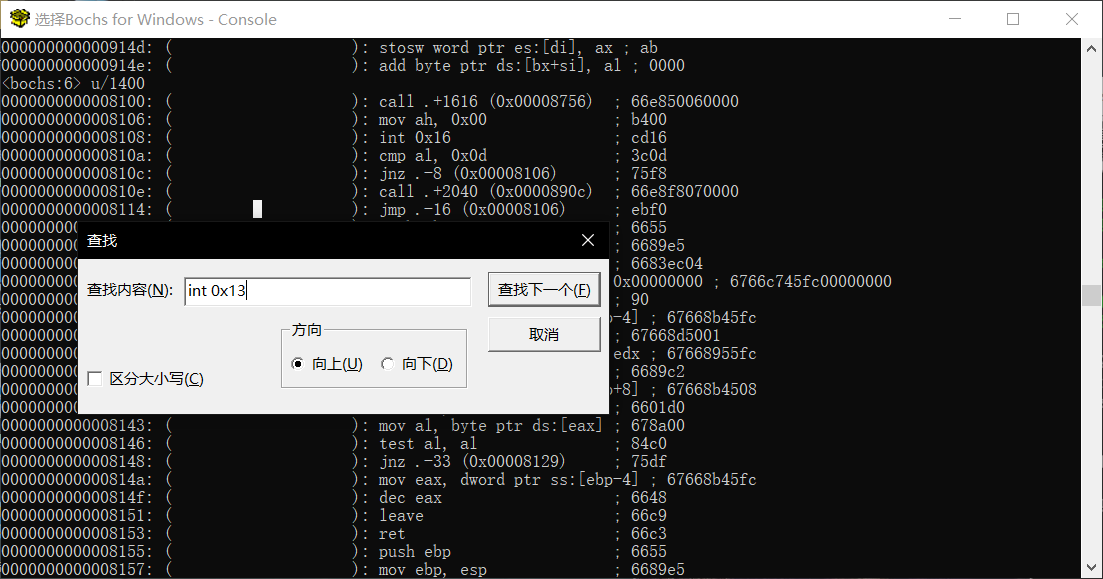
\includegraphics[width=0.8\linewidth]{bochsdbg1.png}
  \caption{用bochs debug过程1}
  \label{fig:bochsdbg1}
\end{figure}
\begin{figure}[H]
  \centering
  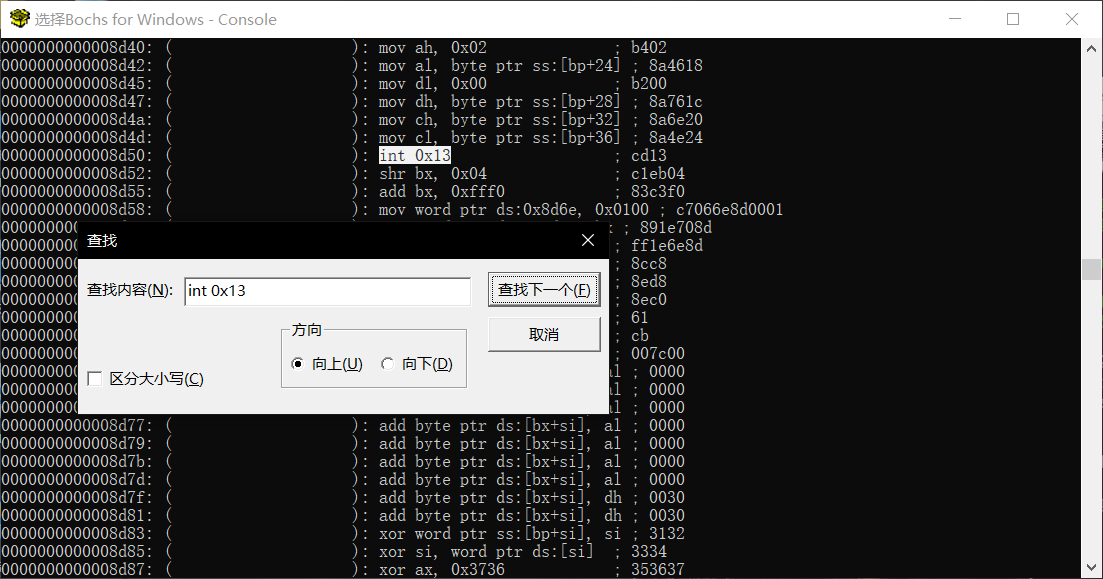
\includegraphics[width=0.8\linewidth]{bochsdbg2.png}
  \caption{用bochs debug过程2}
  \label{fig:bochsdbg2}
\end{figure}
\begin{figure}[H]
  \centering
  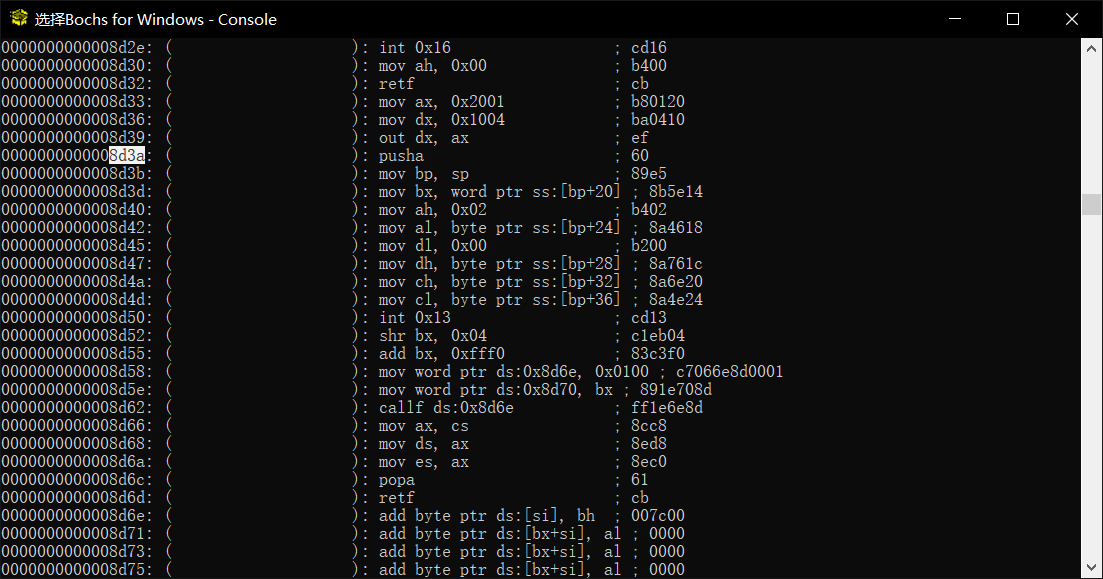
\includegraphics[width=0.8\linewidth]{bochsdbg3.png}
  \caption{用bochs debug过程3}
  \label{fig:bochsdbg3}
\end{figure}
\begin{figure}[H]
  \centering
  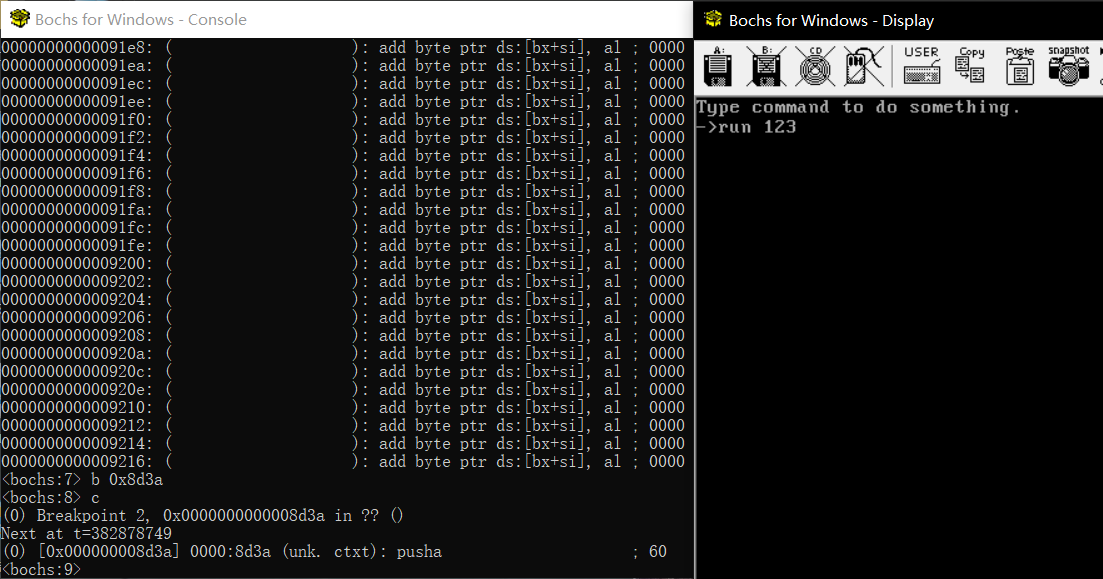
\includegraphics[width=0.8\linewidth]{bochsdbg4.png}
  \caption{用bochs debug过程4}
  \label{fig:bochsdbg4}
\end{figure}
\begin{figure}[H]
  \centering
  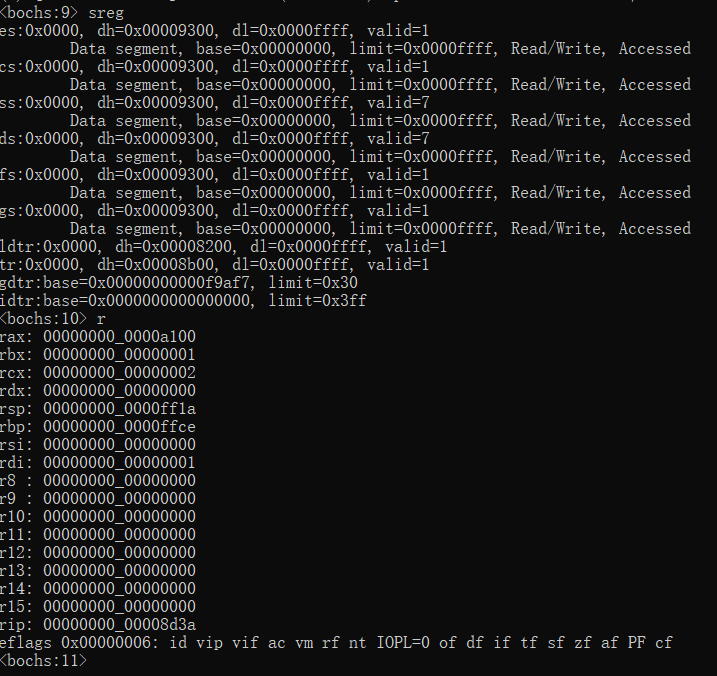
\includegraphics[width=0.8\linewidth]{bochsdbg5.png}
  \caption{用bochs debug过程5}
  \label{fig:bochsdbg5}
\end{figure}

\begin{thebibliography}{99}
  
	\bibitem{lamport94}
  Leslie Lamport,
  \textit{\LaTeX: a document preparation system},
  Addison Wesley, Massachusetts,
  2nd edition,
  1994.
  \bibitem{cite}
  Contributors to Wikibooks,
  \textit{LaTeX Bibliography Management.}
  Wikibooks,
  2019., \\
  en.wikibooks.org/wiki/LaTeX/Bibliography\_Management.
  \bibitem{wikiv8086}
  Virtual 8086 mode
  \textit{Virtual 8086 mode, Wikipedia, The Free Encyclopedia}
  2019., \\
  https://en.wikipedia.org/wiki/Virtual\_8086\_mode
  \bibitem{wikipmode}
  Virtual 8086 mode
  \textit{保护模式, Wikipedia, The Free Encyclopedia}
  2019., \\
  https://zh.wikipedia.org/wiki/%E4%BF%9D%E8%AD%B7%E6%A8%A1%E5%BC%8F
  \bibitem{wikirmode}
  Virtual 8086 mode
  \textit{实模式, Wikipedia, The Free Encyclopedia}
  2019., \\
  https://zh.wikipedia.org/wiki/%E7%9C%9F%E5%AF%A6%E6%A8%A1%E5%BC%8F    
  \bibitem{makefile}
  how-to-write-makefile
  \textit{跟我一起写Makefile}
  陈皓
  2020., \\
  https://seisman.github.io/how-to-write-makefile/overview.html
  \bibitem{realmodedownside}
  Leslie Lamport,
  \textit{操作系统真象还原},
  郑钢,人民邮电出版社
  2016., \\
 
\end{thebibliography}

\section{附录}
\FloatBarrier

% Please add the following required packages to your document preamble:
% \usepackage[table,xcdraw]{xcolor}
% If you use beamer only pass "xcolor=table" option, i.e. \documentclass[xcolor=table]{beamer}
\begin{table}[]
  \caption{项目变量表}
  \label{tab:varlist}
  \begin{tabular}{llll}
  \cellcolor[HTML]{FFFFFF}{\color[HTML]{000000} \textbf{变量声明}} & \cellcolor[HTML]{FFFFFF}{\color[HTML]{000000} \textbf{内容}}         & \cellcolor[HTML]{FFFFFF}{\color[HTML]{000000} \textbf{类型}} & {\color[HTML]{000000} 功能}    \\
  \cellcolor[HTML]{FFFFFF}{\color[HTML]{000000} checknum}      & \cellcolor[HTML]{FFFFFF}{\color[HTML]{000000} 检查是不是合法数字(是数字且在范围内)} & \cellcolor[HTML]{FFFFFF}{\color[HTML]{000000} 函数}          & {\color[HTML]{000000} 格式检查}  \\
  \cellcolor[HTML]{F8F8F8}{\color[HTML]{000000} find}          & \cellcolor[HTML]{F8F8F8}{\color[HTML]{000000} 寻找字符串中特定字符的位置}       & \cellcolor[HTML]{F8F8F8}{\color[HTML]{000000} 函数}          & {\color[HTML]{000000} 字符串操作} \\
  \cellcolor[HTML]{FFFFFF}{\color[HTML]{000000} isnum}         & \cellcolor[HTML]{FFFFFF}{\color[HTML]{000000} 判断是不是数字}             & \cellcolor[HTML]{FFFFFF}{\color[HTML]{000000} 函数}          & {\color[HTML]{000000} 格式检查}  \\
  \cellcolor[HTML]{F8F8F8}{\color[HTML]{000000} printchar}     & \cellcolor[HTML]{F8F8F8}{\color[HTML]{000000} 在光标处重复打印同一字符}        & \cellcolor[HTML]{F8F8F8}{\color[HTML]{000000} 函数}          & {\color[HTML]{000000} IO}    \\
  \cellcolor[HTML]{F8F8F8}{\color[HTML]{000000} printPos}      & \cellcolor[HTML]{F8F8F8}{\color[HTML]{000000} 在某一位置打印字符串}          & \cellcolor[HTML]{F8F8F8}{\color[HTML]{000000} 函数}          & {\color[HTML]{000000} IO}    \\
  \cellcolor[HTML]{FFFFFF}{\color[HTML]{000000} putchar}       & \cellcolor[HTML]{FFFFFF}{\color[HTML]{000000} 在光标处打印单个字符}          & \cellcolor[HTML]{FFFFFF}{\color[HTML]{000000} 函数}          & {\color[HTML]{000000} IO}    \\
  {\color[HTML]{000000} split}                                 & {\color[HTML]{000000} 将字符串在第一个空格处分开成两个}                            & {\color[HTML]{000000} 函数}                                & {\color[HTML]{000000} 字符串操作} \\
  {\color[HTML]{000000} strcmp}                                & {\color[HTML]{000000} 比较两个字符串的大小}                                  & {\color[HTML]{000000} 函数}                                & {\color[HTML]{000000} 字符串操作} \\
  {\color[HTML]{000000} strlen}                                & {\color[HTML]{000000} 计算字符串长度}                                     & {\color[HTML]{000000} 函数}                                & {\color[HTML]{000000} 字符串操作} \\
  {\color[HTML]{000000} cls}                                   & {\color[HTML]{000000} 清屏}                                          & {\color[HTML]{000000} 汇编过程}                                & {\color[HTML]{000000} IO}    \\
  {\color[HTML]{000000} getch}                                 & {\color[HTML]{000000} 获得一个键盘输入}                                    & {\color[HTML]{000000} 汇编过程}                                & {\color[HTML]{000000} IO}    \\
  {\color[HTML]{000000} shutdown}                              & {\color[HTML]{000000} 强制关机}                                        & {\color[HTML]{000000} 汇编过程}                                & {\color[HTML]{000000} 特殊功能}  \\
  {\color[HTML]{000000} loadUsrProgram}                        & {\color[HTML]{000000} 加载并运行用户程序}                                   & {\color[HTML]{000000} 汇编过程}                                & {\color[HTML]{000000} IO}    \\
  {\color[HTML]{000000} Greet}                                 & {\color[HTML]{000000} 打印欢迎信息}                                      & {\color[HTML]{000000} 函数}                                  & {\color[HTML]{000000} 交互}    \\
  {\color[HTML]{000000} middlecol}                             & {\color[HTML]{000000} 计算居中打印的位置}                                   & {\color[HTML]{000000} 函数}                                  & {\color[HTML]{000000} }      \\
  {\color[HTML]{000000} printDetail}                           & {\color[HTML]{000000} 打印软盘中用户程序信息}                                 & {\color[HTML]{000000} 函数}                                  & {\color[HTML]{000000} IO}    \\
  {\color[HTML]{000000} printlnfo}                             & {\color[HTML]{000000} 打印欢迎提示信息}                                    & {\color[HTML]{000000} 函数}                                  & {\color[HTML]{000000} IO}    \\
  {\color[HTML]{000000} printMiddle}                           & {\color[HTML]{000000} 居中打印字符串}                                     & {\color[HTML]{000000} 函数}                                  & {\color[HTML]{000000} IO}    \\
  {\color[HTML]{000000} prompt}                                & {\color[HTML]{000000} 打印'-\textgreater{}'}                         & {\color[HTML]{000000} 函数}                                  & {\color[HTML]{000000} 交互}    \\
  {\color[HTML]{000000} readbuff}                              & {\color[HTML]{000000} 获取用户回车前的完整输入}                                & {\color[HTML]{000000} 函数}                                  & {\color[HTML]{000000} IO}    \\
  {\color[HTML]{000000} newline}                               & {\color[HTML]{000000} 新起一行}                                        & {\color[HTML]{000000} 宏}                                   & {\color[HTML]{000000} IO}    \\
  {\color[HTML]{000000} OffsetOfUserPrg 1}                     & {\color[HTML]{000000} 用户程序1地址偏移量}                                  & {\color[HTML]{000000} 宏}                                   & {\color[HTML]{000000} 保存信息}  \\
  {\color[HTML]{000000} OffsetOfUserPrg2}                      & {\color[HTML]{000000} 用户程序2地址偏移量}                                  & {\color[HTML]{000000} 宏}                                   & {\color[HTML]{000000} 保存信息}  \\
  {\color[HTML]{000000} OffsetOfUserPrg3}                      & {\color[HTML]{000000} 用户程序3地址偏移量}                                  & {\color[HTML]{000000} 宏}                                   & {\color[HTML]{000000} 保存信息}  \\
  {\color[HTML]{000000} OffsetOfUserPrg4}                      & {\color[HTML]{000000} 用户程序4地址偏移量}                                  & {\color[HTML]{000000} 宏}                                   & {\color[HTML]{000000} 保存信息}  \\
  {\color[HTML]{000000} sector}                                & {\color[HTML]{000000} 用户程序信息表结构体}                                  & {\color[HTML]{000000} 结构体}                                 & {\color[HTML]{000000} 保存信息}  \\
  {\color[HTML]{000000} }                                      & {\color[HTML]{000000} }                                            & {\color[HTML]{000000} }                                    &                             
  \end{tabular}
  \end{table}

\begin{lstlisting}[language={[x86masm]Assembler},label=getch,caption=getch]
getch:
    mov ah,0
    int 16h
    mov ah,0
    retf
\end{lstlisting}

\begin{lstlisting}[language={c},label=split,caption=split]
void split(char*buff,char*dest1,char*dest2){
    dest2[0] = '\0';
    int len = strlen(buff);
    int n = find(buff, len, ' ');
    if(n==len-1)
      n = len;
    int i;
    for (i = 0; i < n; i++)
    {
      dest1[i] = buff[i];
    }
    dest1[i] = '\0';
    while (buff[i]&&buff[i]==' ')
    {
      i++;
    }
    int j = 0;
    while(buff[i]){
      dest2[j++] = buff[i++];
    }
    dest2[j] = '\0';
  }
\end{lstlisting}

\begin{lstlisting}[language={c},label=getch,caption=getch]
int find(char *buff, int len, char c)
{
    if (buff[len] != '\0')
      return 0;
    int i = 0;
    while (i < len && buff[i++] != c)
      ;
    return i - 1;
}
\end{lstlisting}

\begin{lstlisting}[language={c},label=strcmp,caption=strcmp]
int find(char *buff, int len, char c)
int strcmp(char *lhs, char *rhs)
{
    int i = 0;
    while (1)
    {
      if (lhs[i] == '\0' || rhs[i] == '\0')
        break;
      if (lhs[i] != rhs[i])
        break;
      ++i;
    }
    return lhs[i] - rhs[i];
}
\end{lstlisting}
  
\begin{lstlisting}[language={[x86masm]Assembler},label=loadUsrProgram,caption=强制关机]
  loadUsrProgram:           
      pusha
      mov bp, sp
      mov bx, [bp+20]        ; 偏移地址; 存放数据的内存偏移地址
      mov ah,2               ; 功能号
      mov al,[bp+24]         ; 扇区数
      mov dl,0               ; 驱动器号; 软盘为0,硬盘和U盘为80H
      mov dh,[bp+28]          ; 磁头号; 起始编号为0
      mov ch,[bp+32]            ; 柱面号; 起始编号为0
      mov cl,[bp+36]          ; 起始扇区号 ; 起始编号为1
      int 13H; 调用读磁盘BIOS的13h功能
      shr bx,4
      add bx,-10h
      mov word[program],0x100
      mov  word[program+2],bx
      call far [program]
      mov ax,cs
      mov ds,ax
      mov es,ax
      popa
      retf
  \end{lstlisting}

\begin{lstlisting}[language={[x86masm]Assembler},label=str.o,caption=str.o]
.file	"str.c"
.code16gcc
.text
.globl	msg
.section	.rodata
.LC0:
	.string	"wodemsg1"
	.data
	.align 4
	.type	msg, @object
	.size	msg, 4
msg:
	.long	.LC0
	.text
	.globl	strlen
	.type	strlen, @function
.LFE0:
	.size	strlen, .-strlen
	.section	.rodata
.LC1:
	.string	"wodeinfo"
	.text
	.globl	printInfo
	.type	printInfo, @function
.LFE1:
	.size	printInfo, .-printInfo
	.globl	printmsg
	.type	printmsg, @function
printmsg:
.LFB2:
	.cfi_startproc
	pushl	%ebp
	.cfi_def_cfa_offset 8
	.cfi_offset 5, -8
	movl	%esp, %ebp
	.cfi_def_cfa_register 5
	subl	$8, %esp
	movl	$9, -4(%ebp)
	movl	$23, -8(%ebp)
	movl	msg, %eax
	pushl	%eax
	call	strlen
	addl	$4, %esp
	movl	%eax, %edx
	movl	msg, %eax
	pushl	-8(%ebp)
	pushl	-4(%ebp)
	pushl	%edx
	pushl	%eax
	call	printPos
	addl	$16, %esp
	nop
	leave
	.cfi_restore 5
	.cfi_def_cfa 4, 4
	ret
	.cfi_endproc
.LFE2:
	.size	printmsg, .-printmsg
	.ident	"GCC: (Ubuntu 7.5.0-3ubuntu1~18.04) 7.5.0"
	.section	.note.GNU-stack,"",@progbits

\end{lstlisting}


%----------------------------------------------------------------------------------------

\end{document}